\subsubsection{Routing information}
\label{sec:sphinx:routinginformation}

Each node on the path needs to decide whether it is destined to be the receiver of the packet and if not, to whom it is supposed to forward it. To achieve the \lcnameref{sec:intro:securitygoals}, each node must only know its direct successor and is allowed to know its predecessor. More precisely, the node must not be able to determine where the next downstream node will forward the packet to, or indeed whether it is the final recipient. Nor should a node know where the packet came from before being sent to its predecessor, or whether its predecessor is the creator of the packet.

This is achieved by applying multiple layers of blinding which are sequentially removed layer by layer at each hop such that the address of the next hop is only visible for one hop along the path.

To ensure that the header has not been tampered while travelling through and network and been transformed by the nodes along the path, an integrity tag is sent in addition to the public key of the next hop. The routing information is thus given by $(y_i, \gamma_i)$, where $y_i$ denotes the public key and $\gamma_i$ the integrity tag for the next downstream node. See Section \ref{sec:sphinx:integrity} for more details on this integrity scheme.

\paragraph{Addresses}

Nodes in the network are distinguished by the ECDSA public keys\footnote{TODO: Add reference}, hence the header includes the public key of the next downstream node and in case of the very last node, a distinguished byte sequence $END$.

ECDSA public keys are given by tuple of two 32-byte field elements $(x,y)$, upon which it is sufficient to solely store the first component $x$ and the sign of $y$, resulting in a \textsf{compressed} elliptic curve point \textsf{0x02}\textless\textsf{x}\textgreater{} for positive $y$ and \textsf{0x03}\textless\textsf{x}\textgreater{} otherwise. The sequence $END$ is given as \textsf{0x04} such that the last node can ignore all subsequent bytes if $END$ is present.

\paragraph{Blinding}

The header uses multiple blindings and their aggregations to make certain sections of the header visible to only a single node. Blindings are generated by a pseudorandomness generator (PRG). See Appendix \ref{appendix:prg} for a detailed description of the PRG employed.

As a result of the Diffie-Hellman key exchange performed in Section \ref{sec:sphinx:keyderivation}, each node along the path can derive a shared secret $s_i$ with the creator of the packet and is therefore able to derive a sub-key $s_i^{bl}$. Both the creator of the packet and each node $n_i$ along the path use $s_i^{bl}$ as a seed for the PRG, yielding $blinding_i$.

The routing information for each node $n_i$ is blinded by XORing the content with $blinding_i$ as well as the blindings $blinding_0, \dots , blinding_{i-1}$ of all previous hops. Each node that receives the packet removes their own blinding from the header and is thus able to extract the routing information destined for them. By removing the blinding from the header, the next downstream node can extract their routing information since it is now only blinded by their blinding.

\paragraph{Example}

The following assumes the sender $A$ is generating routing information for $B, C, D, Z$ and applies their corresponding blinding before sending the header to the first relayer, $B$. The blindings are visualized by different hatchings.\footnote{TODO: Find a clearer visualization scheme.}

\begin{figure}[H]
    \centering
    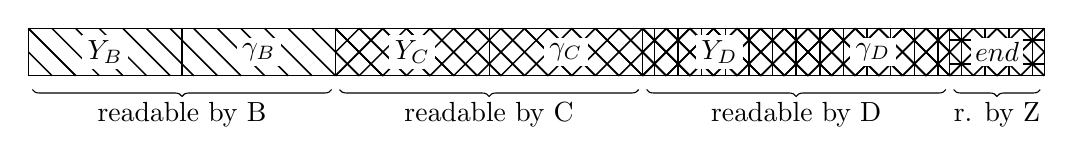
\begin{tikzpicture}
        \def\one{0.6}
        \def\scale{0.9}
        \def\nodeWidth{1.95}
        \def\endWidth{1.2}
        \def\width{3*2*\nodeWidth+\endWidth}
        \foreach \i\name in{0/B,1/C,2/D,3/Z} {
                \begin{scope}[shift={(\i*\nodeWidth*2,0)}]
                    \ifnum\i=0
                        \def\a{11.7}
                        \def\diff{11.1}
                    \fi

                    \ifnum\i=1
                        \def\a{7.8}
                        \def\diff{7.2}
                    \fi

                    \ifnum\i=2
                        \def\a{3.9}
                        \def\diff{3.3}

                    \fi

                    \ifnum\i=3
                        \def\a{\endWidth}
                        \def\diff{0.6}
                    \fi


                    \def\b{\one}
                    \def\lw{0.2}

                    \foreach \x [count=\i] in{0,0.3,0.6,...,\b}{
                            \draw [line width=\lw mm](\x,0)--(0,\x) (\a-\b+\x,\b)--(\a,\x);
                        }
                    \foreach \x [count=\i] in{0,0.3,0.6,...,\diff}{
                            \draw [line width=\lw mm](\x+\b,0)--(\x,\b);
                        }

                    \ifnum\i>0
                        \foreach \x [count=\i] in{0,0.3,0.6,...,\b}{
                                \draw [line width=\lw mm](0,\x)--(\b-\x,\b) (\a-\b+\x,0)--(\a,\b-\x);
                            }
                        \foreach \x [count=\i] in{0,0.3,0.6,...,\diff}{
                                \draw [line width=\lw mm](\x,0)--(\b+\x,\b);
                            }
                    \fi

                    \ifnum\i>1
                        \foreach \x [count=\i] in{0.15,0.45,...,\a}{
                                \draw [line width=\lw mm](\x,0)--(\x,\b);
                            }
                    \fi

                    \ifnum\i>2
                        \foreach \x [count=\i] in{0.15,0.45,...,\b}{
                                \draw [line width=\lw mm](0,\x)--(\a,\x);
                            }
                    \fi
                \end{scope}
                \ifnum\i<3
                    \draw [color=white] (\i*2*\nodeWidth,0) rectangle (\i*2*\nodeWidth+\nodeWidth,\one) node [midway,color=black,fill=white,inner sep=2pt] {$Y_{\name}$};
                    \draw (\i*2*\nodeWidth,0) -- (\i*2*\nodeWidth,\one);
                    \draw [color=white] (\i*2*\nodeWidth+\nodeWidth,0) rectangle (\i*2*\nodeWidth+2*\nodeWidth,\one) node [midway,color=black,fill=white,inner sep=2pt] {$\gamma_{\name}$};
                    \draw (\i*2*\nodeWidth+\nodeWidth,0) -- (\i*2*\nodeWidth+\nodeWidth,\one);

                    \draw[decoration={brace,raise=5pt,mirror},decorate] (\nodeWidth*2*\i+0.05,0) -- (\nodeWidth*2*\i+\nodeWidth*2-0.05,0) node[midway,below=6pt] {readable by \name};
                \else
                    \draw [color=white] (\i*2*\nodeWidth,0) rectangle (\i*2*\nodeWidth+\endWidth,\one) node [midway,color=black,fill=white,inner sep=1.5pt] {$end$};
                    \draw (\i*2*\nodeWidth,0) -- (\i*2*\nodeWidth,\one);

                    \draw[decoration={brace,raise=5pt,mirror},decorate] (\i*2*\nodeWidth+0.05,0) -- (\i*2*\nodeWidth+\endWidth-0.05,0) node[midway,below=6pt] {r. by \name};
                \fi
            }

        \draw (0,0) rectangle (\width,\one);
    \end{tikzpicture}
    \caption{Blinded routing information sent to first relayer $B$.}
\end{figure}